%==========================================================================
%  TRES0312 Fysikk — Foiler-mal
%
%  Mørk/lys modus: kommenter ut én av de to linjene nedenfor.
%==========================================================================
\newif\ifdarkmode
\darkmodetrue      % ← mørk modus
%\darkmodefalse   % ← lys modus  (fjern % foran og legg % foran linjen over)

\documentclass[aspectratio=169, 12pt]{beamer}

\usepackage{amd-beamer}

%--------------------------------------------------------------------------
%  FIGURFARER — god kontrast i både mørk og lys modus
%--------------------------------------------------------------------------
\ifdarkmode
  \colorlet{figA}   {cyan!80!white}      % knallcyan   — vektor A / hoved
  \colorlet{figB}   {green!80!lime}      % knallgrønn  — vektor B
  \colorlet{figC}   {orange}             % oransje     — resultantvektor
  \colorlet{figProj}{yellow!90!white}    % gul         — projeksjon / cos
  \colorlet{figFill}{cyan!18!black}      % svak cyan   — fyllfarge
\else
  \colorlet{figA}   {teal!85!black}      % dyp teal
  \colorlet{figB}   {green!60!black}     % mørk grønn
  \colorlet{figC}   {orange!90!red}      % oransje-rød
  \colorlet{figProj}{orange!75!yellow}   % rav
  \colorlet{figFill}{teal!14!white}      % lys teal
\fi

%--------------------------------------------------------------------------
%  DOKUMENTINFO
%--------------------------------------------------------------------------
\title{Matematikk vi trenger!}
\subtitle{TRES0312 --- Kapittel 2}
\author{Ben David Normann}
\date{\today}

%--------------------------------------------------------------------------
%  SEKSJONSKONTEKST
%  Setter kapittelteller til 2 slik at nummerering matcher kompendiet.
%--------------------------------------------------------------------------
\setcounter{section}{2}

\begin{document}

%--------------------------------------------------------------------------
%  SLIDE 1 — TITTELSIDE
%--------------------------------------------------------------------------
\begin{frame}[plain]
  \titlepage
\end{frame}

%--------------------------------------------------------------------------
%  SLIDE 2 — DAGENS PLAN
%--------------------------------------------------------------------------
\begin{frame}{Dagens plan}
  \begin{columns}[t]
    \begin{column}{0.48\textwidth}
      \oppsum{Del 1 — 45 min}{%
        \begin{itemize}
          \item Algebra-regler
          \item Funksjoner og plotting
          \item Trigonometri
        \end{itemize}
      }
    \end{column}
    \begin{column}{0.48\textwidth}
      \oppsum{Del 2 — 45 min}{%
        \begin{itemize}
          \item Vektorer
          \item Koordinatsystem og enhetsvektorer
          \item Størrelse og retning
          \item Vektoroperasjoner
        \end{itemize}
      }
    \end{column}
  \end{columns}
\end{frame}

%--------------------------------------------------------------------------
%  SLIDE 3 — ALGEBRAREGLER
%--------------------------------------------------------------------------
\begin{frame}{Algebra}
  \oppsum{Algebraregler}{%
    \begin{itemize}
      \item Det du gjør på ett ledd, gjør du på \textit{alle} ledd i likningen.
      \item \textbf{Potenser:} $x^a \cdot x^b = x^{a+b}$, \quad
            $\dfrac{x^a}{x^b} = x^{a-b}$, \quad $(x^a)^b = x^{ab}$.
      \item \textbf{Kvadratsetninger:}
            $(a+b)^2 = a^2+2ab+b^2$, \quad
            $(a-b)^2 = a^2-2ab+b^2$,\\[2pt]
            $(a+b)(a-b)=a^2-b^2$.
    \end{itemize}
  }
  \pause
  \aktivitet{Løs for den ukjente}{%
    \begin{enumerate}[a)]
      \item Finn $a$: \quad $F = m\cdot a$, \quad $F = 4\,800\ \mathrm{N}$,
            \quad $m = 1\,200\ \mathrm{kg}$.
      \item Finn $v$: \quad $E_K = \tfrac{1}{2}mv^2$, \quad $E_K = 25\ \mathrm{J}$,
            \quad $m = 2{,}0\ \mathrm{kg}$.
    \end{enumerate}
  }
\end{frame}

%--------------------------------------------------------------------------
%  SLIDE 4 — ALGEBRA OPPGAVE
%--------------------------------------------------------------------------
\begin{frame}{Oppgave}
  \aktivitet{Algebra}{%
    \begin{enumerate}[a)]
      \item Regn ut: $\dfrac{15 + 3^2}{6-2}$.
      \item Forenkle: $\dfrac{x^4 \cdot x^{-2}}{x^3}$.
      \item Løs for $t$: \quad $s = \tfrac{1}{2}at^2$, \quad
            $s = 20\ \mathrm{m}$, \quad $a = 10\ \mathrm{m/s}^2$.
    \end{enumerate}
  }
\end{frame}

%--------------------------------------------------------------------------
%  SLIDE 5 — FUNKSJONER
%--------------------------------------------------------------------------
\begin{frame}{Funksjoner}
  \spq{Hva er en funksjon?}
  \pause
  \svar{En funksjon $f$ knytter til enhver innverdi $x$ én bestemt utverdi $f(x)$.}
  \pause
  \oppsum{Viktige typer}{%
    \begin{itemize}
      \item \textbf{Lineær:} $f(x) = b + ax$
            \quad — f.eks.\ $v(t) = v_0 + at$
      \item \textbf{Kvadratisk:} $f(x) = ax^2 + bx + c$
            \quad — f.eks.\ $s(t) = \tfrac{1}{2}at^2 + v_0 t + s_0$
    \end{itemize}
  }
\end{frame}

%--------------------------------------------------------------------------
%  SLIDE 6 — FIGUR 2.1
%--------------------------------------------------------------------------
\begin{frame}{Funksjoner: eksempel fra bevegelse}
  \begin{center}
    \includegraphics[width=0.93\textwidth, keepaspectratio]%
      {Kapittel1:introduksjon/python_plot_02_bevegelse.pdf}\\[0.3em]
    {\small Figur~2.1: Posisjon og fart som funksjon av tid for konstant akselerasjon
    $a=2{,}0\ \mathrm{m/s}^2$, $v_0=0$.}
  \end{center}
\end{frame}

%--------------------------------------------------------------------------
%  SLIDE 7 — TRIGONOMETRI: RETTVINKLET TREKANT
%--------------------------------------------------------------------------
\begin{frame}{Trigonometri}
  \begin{columns}[c]
    \begin{column}{0.46\textwidth}
      \begin{center}
      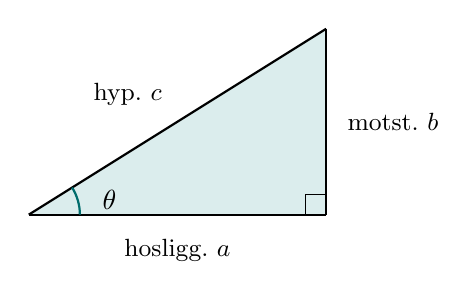
\begin{tikzpicture}[scale=1.18]
        \coordinate (O) at (0,0);
        \coordinate (A) at (3.2,0);
        \coordinate (B) at (3.2,2.0);
        \fill[figFill] (O)--(A)--(B)--cycle;
        \draw[thick](O)--(A)
              node[midway, below=5pt]{\small hosligg.\ $a$};
        \draw[thick](A)--(B)
              node[midway, right=4pt]{\small motst.\ $b$};
        \draw[thick](O)--(B)
              node[midway, above left=2pt]{\small hyp.\ $c$};
        \draw (A)++(-0.22,0)--++(0,0.22)--++(0.22,0);
        \draw[figA, thick](0.55,0) arc(0:32:0.55);
        \node at (0.87,0.16){$\theta$};
      \end{tikzpicture}
      \end{center}
    \end{column}
    \begin{column}{0.52\textwidth}
      \oppsum{Definisjoner}{%
        \[
          \cos\theta = \frac{a}{c}, \quad
          \sin\theta = \frac{b}{c}, \quad
          \tan\theta = \frac{b}{a}
        \]
        \medskip
        \textbf{Komponenter:}
        \[
          a = c\cos\theta, \qquad b = c\sin\theta
        \]
      }
    \end{column}
  \end{columns}
\end{frame}

%--------------------------------------------------------------------------
%  SLIDE 8 — ENHETSSIRKELEN
%--------------------------------------------------------------------------
\begin{frame}{Enhetssirkelen}
  \begin{columns}[c]
    \begin{column}{0.44\textwidth}
      \begin{center}
      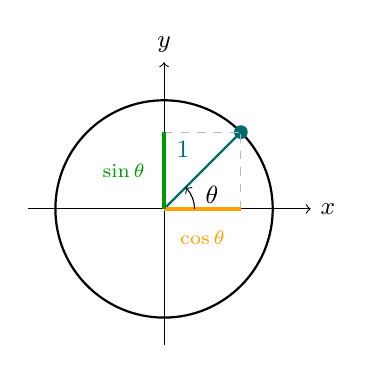
\begin{tikzpicture}[scale=1.38]
        \draw[->](-1.25,0)--(1.35,0) node[right, font=\small]{$x$};
        \draw[->](0,-1.25)--(0,1.35) node[above, font=\small]{$y$};
        \draw[thick](0,0) circle(1);
        \fill[figA](0.707,0.707) circle(1.8pt);
        \draw[thick, figA](0,0)--(0.707,0.707)
              node[midway, above left=1pt, font=\small]{$1$};
        \draw[dashed, gray!55](0.707,0)--(0.707,0.707);
        \draw[dashed, gray!55](0,0.707)--(0.707,0.707);
        \draw[very thick, figProj](0,0)--(0.707,0)
              node[midway, below=4pt, font=\scriptsize]{$\cos\theta$};
        \draw[very thick, figB](0,0)--(0,0.707)
              node[midway, left=3pt, font=\scriptsize]{$\sin\theta$};
        \draw[->](0.28,0) arc(0:45:0.28);
        \node[font=\small] at (0.44,0.13){$\theta$};
      \end{tikzpicture}
      \end{center}
    \end{column}
    \begin{column}{0.52\textwidth}
      \renewcommand{\arraystretch}{1.35}
      \begin{center}\scriptsize
      \begin{tabular}{|c|c|c|c|}
      \hline
      \rowcolor{blue!10!black!80}
      $\theta$ & $\sin\theta$ & $\cos\theta$ & $\tan\theta$ \\
      \hline
      $0^\circ$  & $0$ & $1$ & $0$ \\
      $30^\circ$ & $\frac{1}{2}$ & $\frac{\sqrt{3}}{2}$ & $\frac{1}{\sqrt{3}}$ \\
      $45^\circ$ & $\frac{\sqrt{2}}{2}$ & $\frac{\sqrt{2}}{2}$ & $1$ \\
      $60^\circ$ & $\frac{\sqrt{3}}{2}$ & $\frac{1}{2}$ & $\sqrt{3}$ \\
      $90^\circ$ & $1$ & $0$ & --- \\
      \hline
      \end{tabular}
      \end{center}
      \smallskip
      {\scriptsize\textit{Pythagoras på enhetssirkelen:
      $\cos^2\theta + \sin^2\theta = 1$}}
    \end{column}
  \end{columns}
\end{frame}

%--------------------------------------------------------------------------
%  SLIDE 9 — TRIGONOMETRI OPPGAVE
%--------------------------------------------------------------------------
\begin{frame}{Oppgave}
  \aktivitet{Trigonometri: stige mot vegg}{%
    En stige av lengde $c = 5{,}0\ \mathrm{m}$ lener seg mot en vegg i
    vinkel $\theta = 37^\circ$ med gulvet.
    \begin{enumerate}[a)]
      \item Finn den horisontale komponenten $a$ og den vertikale $b$.
      \item Sjekk svaret ditt med Pythagoras: $a^2 + b^2 = c^2$.
      \item Hva blir $b$ dersom $\theta$ økes til $53^\circ$?
    \end{enumerate}
  }
\end{frame}

%--------------------------------------------------------------------------
%  SLIDE 10 — PAUSE
%--------------------------------------------------------------------------
\begin{frame}{}
  \begin{center}
    \Huge{Pause!}
  \end{center}
\end{frame}

%--------------------------------------------------------------------------
%  SLIDE 11 — VEKTORER
%--------------------------------------------------------------------------
\begin{frame}{Vektorer}
  \spq{Hva er en vektor?}
  \pause
  \svar{Et objekt med både \textit{størrelse} og \textit{retning}.
        Vi skriver $\vec{v}$.}
  \pause
  \begin{center}
  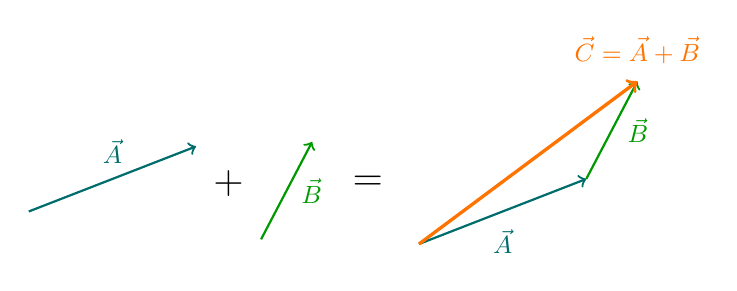
\begin{tikzpicture}[scale=1.18, baseline=(current bounding box.center)]
    %--- Frie vektorer A og B ---
    \draw[->, thick, figA](0,0.35)--(1.8,1.05);
    \node[above=2pt, font=\small, figA] at (0.9,0.70){$\vec{A}$};
    \node[font=\Large] at (2.15,0.65){$+$};
    \draw[->, thick, figB](2.50,0.05)--(3.05,1.10);
    \node[right=2pt, font=\small, figB] at (2.77,0.57){$\vec{B}$};
    %--- Likhetstegn ---
    \node[font=\Large] at (3.65,0.65){$=$};
    %--- Tip-til-hale-addisjon ---
    \draw[->, thick, figA](4.2,0)--(6.0,0.70);
    \node[below=3pt, font=\small, figA] at (5.1,0.35){$\vec{A}$};
    \draw[->, thick, figB](6.0,0.70)--(6.55,1.75);
    \node[right=2pt, font=\small, figB] at (6.28,1.22){$\vec{B}$};
    \draw[->, very thick, figC](4.2,0)--(6.55,1.75);
    \node[above=3pt, font=\small, figC] at (6.55,1.75){$\vec{C}=\vec{A}+\vec{B}$};
  \end{tikzpicture}
  \end{center}
\end{frame}

%--------------------------------------------------------------------------
%  SLIDE 12 — KOORDINATSYSTEM
%--------------------------------------------------------------------------
\begin{frame}{Koordinatsystem}
  \begin{center}
  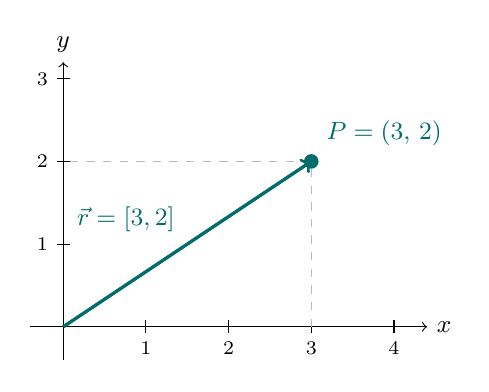
\begin{tikzpicture}[scale=1.05]
    \draw[->](-0.4,0)--(4.4,0) node[right, font=\small]{$x$};
    \draw[->](0,-0.4)--(0,3.2)  node[above, font=\small]{$y$};
    \foreach \x in {1,2,3,4}{%
      \draw(\x,0.08)--(\x,-0.08);
      \node[below=2pt, font=\scriptsize] at (\x,0){$\x$};}
    \foreach \y in {1,2,3}{%
      \draw(0.08,\y)--(-0.08,\y);
      \node[left=2pt, font=\scriptsize] at (0,\y){$\y$};}
    \draw[dashed, gray!55](3,0)--(3,2)--(0,2);
    \draw[->, very thick, figA](0,0)--(3,2);
    \fill[figA](3,2) circle(2.5pt);
    \node[above right=2pt, font=\small, figA] at (3,2){$P=(3,\,2)$};
    \node[above left=1pt, font=\small, figA] at (1.5,1.0){$\vec{r}=[3,2]$};
  \end{tikzpicture}
  \end{center}
  \tanke{}{%
    Et koordinatsystem lar oss beskrive vektorer med komponenter.}
\end{frame}

%--------------------------------------------------------------------------
%  SLIDE 13 — ENHETSVEKTORER
%--------------------------------------------------------------------------
\begin{frame}{Enhetsvektorer}
  \oppsum{Enhetsvektorer og komponentform}{%
    I $xy$-planet: \quad
    $\hat{\mathbf{x}} = [1,0]$ \quad og \quad $\hat{\mathbf{y}} = [0,1]$.\\[0.6em]
    Enhver vektor kan skrives på to ekvivalente måter:
    \[
      \vec{v} = [v_x,\,v_y] = v_x\hat{\mathbf{x}} + v_y\hat{\mathbf{y}}
    \]
  }
  \pause
  \aktivitet{Komponentform}{%
    \begin{enumerate}[a)]
      \item Skriv $\vec{A} = [4,\,-3]$ som en lineær kombinasjon
            av $\hat{\mathbf{x}}$ og $\hat{\mathbf{y}}$.
      \item Regn ut $\vec{u}+\vec{v}$ der $\vec{u} = 3\hat{\mathbf{x}}-2\hat{\mathbf{y}}$
            og $\vec{v} = -\hat{\mathbf{x}}+5\hat{\mathbf{y}}$.
    \end{enumerate}
  }
\end{frame}

%--------------------------------------------------------------------------
%  SLIDE 14 — STØRRELSE OG RETNING
%--------------------------------------------------------------------------
\begin{frame}{Størrelse og retning}
  \oppsum{Lengde og vinkel til en vektor}{%
    For $\vec{v} = [v_x,\,v_y]$:
    \[
      |\vec{v}| = \sqrt{v_x^2 + v_y^2}, \qquad
      \theta = \arctan\!\left(\frac{v_y}{v_x}\right)
    \]
  }
  \pause
  \aktivitet{Finn størrelse og retning}{%
    Gitt $\vec{v} = [3,\,4]$.
    \begin{enumerate}[a)]
      \item Finn lengden $|\vec{v}|$.
      \item Finn vinkelen $\theta$ med positiv $x$-akse.
    \end{enumerate}
  }
\end{frame}

%--------------------------------------------------------------------------
%  SLIDE 15 — ADDISJON OG SKALARMULTIPLIKASJON
%--------------------------------------------------------------------------
\begin{frame}{Vektoraddisjon og skalarmultiplikasjon}
  \begin{columns}[t]
    \begin{column}{0.48\textwidth}
      \oppsum{Addisjon}{%
        \medskip
        $\vec{u}+\vec{v} = [u_x+v_x,\; u_y+v_y]$
        \medskip
      }
    \end{column}
    \begin{column}{0.48\textwidth}
      \oppsum{Skalarmultiplikasjon}{%
        For en skalar $k$:
        \medskip
        $k\vec{v} = [kv_x,\; kv_y]$
        \medskip\\
        $k>1$: strekker;\; $k<0$: snur retning.
      }
    \end{column}
  \end{columns}
  \pause
  \aktivitet{Regn}{%
    Gitt $\vec{a}=[3,\,-1]$ og $\vec{b}=[-1,\,4]$.
    Finn $\vec{a}+\vec{b}$, \; $\vec{a}-\vec{b}$ \; og \; $2\vec{a}-3\vec{b}$.
  }
\end{frame}

%--------------------------------------------------------------------------
%  SLIDE 16 — SKALARPRODUKT
%--------------------------------------------------------------------------
\begin{frame}{Skalarprodukt (prikkprodukt)}
  \begin{columns}[c]
    \begin{column}{0.46\textwidth}
      \oppsum{Definisjon}{%
        \[
          \begin{aligned}
            \vec{u}\cdot\vec{v}
            &= u_xv_x + u_yv_y \\
            &= |\vec{u}|\,|\vec{v}|\cos\theta
          \end{aligned}
        \]
        \begin{itemize}
          \item Gir en \textit{skalar} (et tall).
          \item $\vec{u}\perp\vec{v}
                \;\Leftrightarrow\; \vec{u}\cdot\vec{v}=0$.
        \end{itemize}
      }
    \end{column}
    \begin{column}{0.50\textwidth}
      \begin{center}
      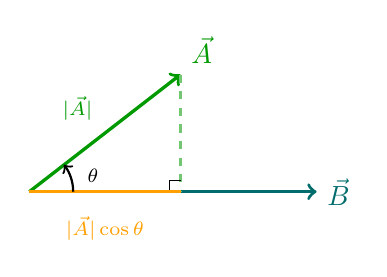
\begin{tikzpicture}[scale=0.96]
        \draw[->, very thick, figA](0,0)--(3.8,0)
              node[right]{$\vec{B}$};
        \draw[->, very thick, figB](0,0)--(2.0,1.55)
              node[above right]{$\vec{A}$};
        \node[above left=1pt, figB, font=\scriptsize]
              at (1.0,0.78){$|\vec{A}|$};
        \draw[dashed, figB!55, thick](2.0,1.55)--(2.0,0);
        \draw (2.0,0)++(-0.15,0)--++(0,0.15)--++(0.15,0);
        \draw[very thick, figProj](0,0)--(2.0,0)
              node[midway, below=5pt, font=\scriptsize]
              {$|\vec{A}|\cos\theta$};
        \draw[->, thick](0.58,0) arc(0:37.87:0.58);
        \node[font=\scriptsize] at (0.84,0.21){$\theta$};
      \end{tikzpicture}
      \end{center}
    \end{column}
  \end{columns}
\end{frame}

%--------------------------------------------------------------------------
%  SLIDE 17 — KRYSSPRODUKT
%--------------------------------------------------------------------------
\begin{frame}{Kryssprodukt}
  \begin{columns}[c]
    \begin{column}{0.46\textwidth}
      \oppsum{Kryssprodukt (2D)}{%
        \[
          \begin{aligned}
            (\vec{u}{\times}\vec{v})_z
            &= u_xv_y - u_yv_x \\
            &= |\vec{u}|\,|\vec{v}|\sin\theta
          \end{aligned}
        \]
        \begin{itemize}
          \item Størrelse = areal av parallellogrammet.
          \item Parallelle vektorer: $\vec{u}\times\vec{v}=0$.
          \item Ikke kommutativt:
                $\vec{u}\times\vec{v} = -\vec{v}\times\vec{u}$.
        \end{itemize}
      }
    \end{column}
    \begin{column}{0.50\textwidth}
      \begin{center}
      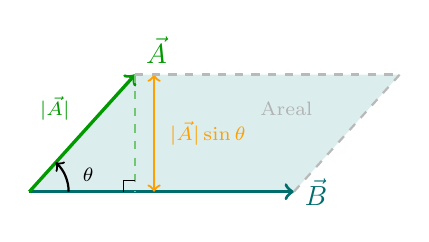
\begin{tikzpicture}[scale=0.96]
        \fill[figFill]
              (0,0)--(3.5,0)--(4.9,1.55)--(1.4,1.55)--cycle;
        \draw[->, very thick, figA](0,0)--(3.5,0)
              node[right]{$\vec{B}$};
        \draw[->, very thick, figB](0,0)--(1.4,1.55)
              node[above right]{$\vec{A}$};
        \node[above left=1pt, figB, font=\scriptsize]
              at (0.7,0.78){$|\vec{A}|$};
        \draw[dashed, figB!55, thick](1.4,1.55)--(1.4,0);
        \draw (1.4,0)++(-0.15,0)--++(0,0.15)--++(0.15,0);
        \draw[<->, thick, figProj](1.65,0)--(1.65,1.55)
              node[midway, right=2pt, font=\scriptsize]
              {$|\vec{A}|\sin\theta$};
        \draw[dashed, gray!55, thick](3.5,0)--(4.9,1.55);
        \draw[dashed, gray!55, thick](1.4,1.55)--(4.9,1.55);
        \node[font=\scriptsize, gray!60] at (3.4,1.1){Areal};
        \draw[->, thick](0.52,0) arc(0:48:0.52);
        \node[font=\scriptsize] at (0.78,0.22){$\theta$};
      \end{tikzpicture}
      \end{center}
    \end{column}
  \end{columns}
\end{frame}

%--------------------------------------------------------------------------
%  SLIDE 18 — OPPGAVER: OPERASJONER
%--------------------------------------------------------------------------
\begin{frame}{Oppgave}
  \begin{columns}[t]
    \begin{column}{0.48\textwidth}
      \aktivitet{Skalarprodukt og vinkel}{%
        Gitt $\vec{u}=[4,\,3]$ og $\vec{v}=[2,\,-1]$.
        \begin{enumerate}[a)]
          \item Finn $\vec{u}\cdot\vec{v}$.
          \item Finn vinkelen mellom $\vec{u}$ og $\vec{v}$.
        \end{enumerate}
      }
    \end{column}
    \begin{column}{0.48\textwidth}
      \aktivitet{Kryssprodukt og areal}{%
        Gitt $\vec{u}=[4,\,1]$ og $\vec{v}=[2,\,3]$.
        \begin{enumerate}[a)]
          \item Finn $(\vec{u}\times\vec{v})_z$.
          \item Hva er arealet av parallellogrammet?
          \item Finn $(\vec{v}\times\vec{u})_z$ og forklar fortegnet.
        \end{enumerate}
      }
    \end{column}
  \end{columns}
\end{frame}

%--------------------------------------------------------------------------
%  SLIDE 19 — AVSLUTNING
%--------------------------------------------------------------------------
\begin{frame}
  \begin{center}
    \Huge{Neste gang: Kapittel 3 --- Kinematikk!}
    \begin{itemize}
      \item Posisjon, hastighet og akselerasjon
      \item Bevegelsesligninger
      \item Fri bevegelse og kast
    \end{itemize}
  \end{center}
\end{frame}

\end{document}
